\section{Classical Runge-Kutta method with adaptive time step}
We consider again the initial value problem in (\ref{2_problem}).
\subsection{Describe the classical Runge-Kutta method with adaptive step size}
The classical Runge-Kutta is described in exercise \ref{5_1}. The only change introduced in this part will be implementing the error estimation using step doubling and the asymptotic step size controller.

%%%%%%%%%%%%%%%%%%%%%%%%%%%%%%%%%%%%%%%%%%%%%%%%%%%%%%%%%%%%%%%%%%%%%%%%%%%%%%%%%%%%%%%%%%%%%%%%%%%
\subsection{Implement an algorithm in Matlab for the classical Runge-Kutta method with adaptive time step size. Provide the code in your report.  Use a format that enables syntax highlighting. Comment on the code}
\begin{lstlisting}[caption = Classical Runge-Kutta method with adaptive time step size, captionpos=b, label=6_ClassicRK4_adaptive]
function [T,X,r_out,h_out,info] = ClassicRK4_adaptive(fun,tspan,h0,x0,abstol,reltol,args)

epstol = 0.8;
kpow = 0.2;
facmin = 0.1;
facmax = 5.0;

t0 = tspan(1);
tf = tspan(end);
t = t0;
h = h0;
x = x0;

T = t0;
X = x0;
r_out = [];
h_out = [];
info = zeros(1,4);

nfun = 0;
nstep = 0;
naccept = 0;

while t < tf
    if (t+h > tf)
        h = tf-t;
    end
    
    nfun = nfun + 1;
    AcceptStep = false;
    while ~AcceptStep
        x1 = ClassicRK4_step(fun,t,h,x,args);
        nfun = nfun + 4;
        
        hm = 0.5*h;
        tm = t + hm;
        xm = ClassicRK4_step(fun,t,hm,x,args);
        nfun = nfun + 4;
        x1hat = ClassicRK4_step(fun,tm,hm,xm,args);
        nfun = nfun + 4;
        nstep = nstep + 1;
        
        e = abs(x1hat-x1);
        r = max(e./max(abstol, abs(x1hat) .* reltol));
        AcceptStep = (r <= 1.0);
        
        if AcceptStep
            t = t+h;
            x = x1hat;
            
            T = [T,t];
            X = [X,x];
            r_out = [r_out, r];
            h_out = [h_out, h];
            naccept = naccept + 1;
        end
        
        h = max(facmin, min((epstol/r)^kpow, facmax)) * h;
    end
end

info(1) = nfun;
info(2) = nstep;
info(3) = naccept;
info(4) = nstep - naccept;

end
\end{lstlisting}

%%%%%%%%%%%%%%%%%%%%%%%%%%%%%%%%%%%%%%%%%%%%%%%%%%%%%%%%%%%%%%%%%%%%%%%%%%%%%%%%%%%%%%%%%%%%%%%%%%%
\subsection{Test your problem for test equation. Discuss order and stability of the numerical method}
Implementing the adaptive classical Runge-Kutta just as we did for the classical one leads us to the results shown below. It's curious to see that the relation between the local and global error vs. the tolerance. The relation between them was found empirically.

The stability of the method is already discussed in Exercise \ref{5_3}.

\begin{figure}[H]
    \centering
    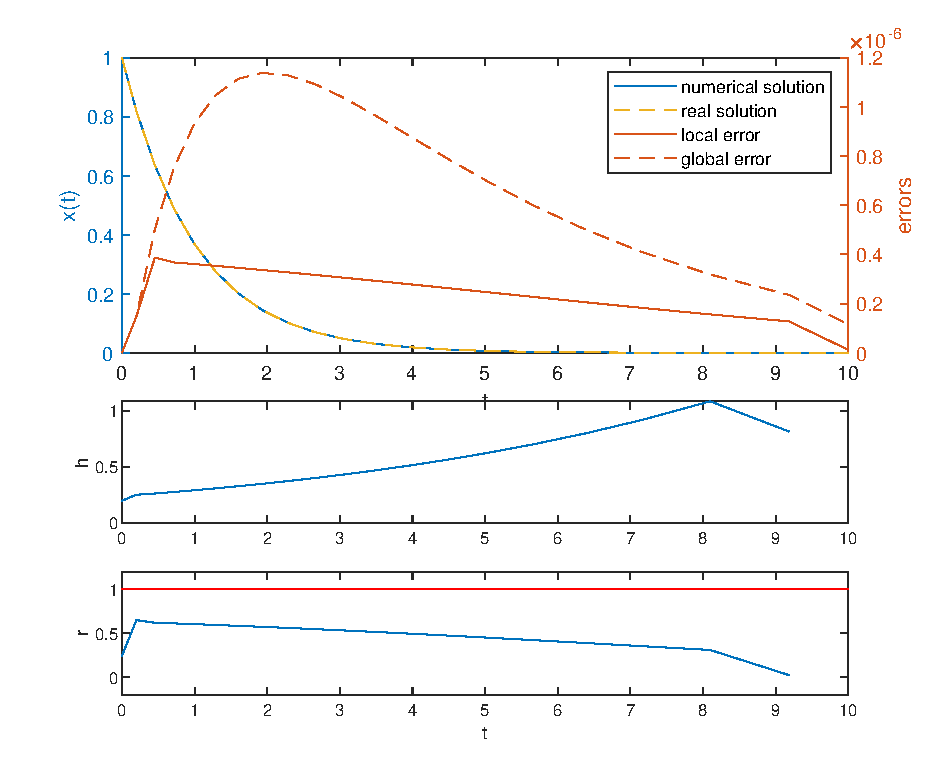
\includegraphics[width=0.7\linewidth]{images/6/6_3_TestEquation.pdf} 
    \caption{Solution and errors vs. time for the Test equation using adaptive classical Runge-Kutta method}
    \label{6_3_TE}
\end{figure}

\begin{figure}[H]
\centering
    \begin{subfigure}{0.49\linewidth}
        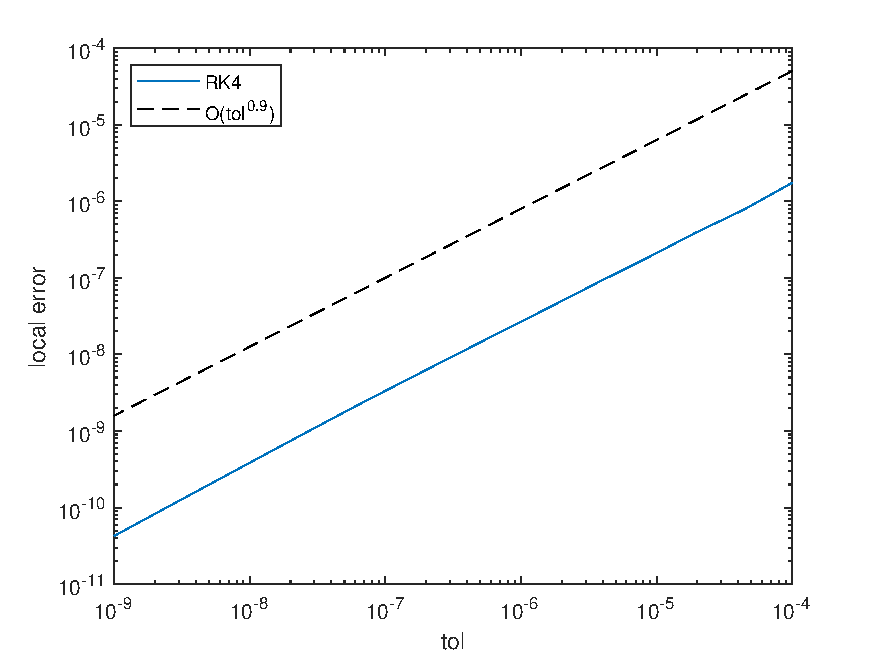
\includegraphics[width=\linewidth]{images/6/6_3_localerror.pdf}
        \caption{Local error}
    \end{subfigure}
    \begin{subfigure}{0.49\linewidth}
        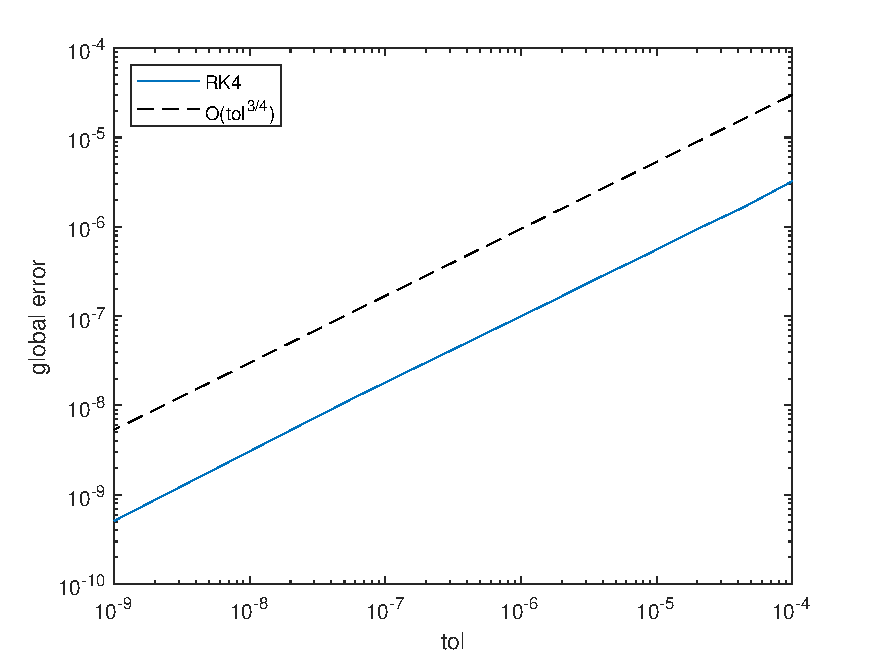
\includegraphics[width=\linewidth]{images/6/6_3_globalerror.pdf}
        \caption{Global error}
    \end{subfigure}
    \caption{Local and global errors vs. time-step size for the Test equation using adaptive classical Runge-Kutta method}
    \label{6_3_TE_errors}
\end{figure}

%%%%%%%%%%%%%%%%%%%%%%%%%%%%%%%%%%%%%%%%%%%%%%%%%%%%%%%%%%%%%%%%%%%%%%%%%%%%%%%%%%%%%%%%%%%%%%%%%%%
\subsection{Test your algorithms on the Van der Pol problem \texorpdfstring{($\mathbf{\mu = 1.5}$ and $\mathbf{\mu = 15}$, $\mathbf{x_0 = [1.0;1.0]}$).}{(mu = 1.5 and mu = 15, x0 = [1.0;1.0]).}}
The results for the Van der pol problem are shown below. When comparing to the Explicit Euler with adaptive results shown in Figures \ref{2_4_adaptive_mu_1_5} and \ref{2_4_adaptive_mu_15}, we can see that the method achieves better performance when working with same tolerances, or even larger. The change of frequency of the signals has disappeared completely and all tolerances approach the real solution pretty good. However, as it's an explicit method, it's still sensible to the stiffness of the Van der Pol with $\mu=15$. Specially, comparing Tables \ref{2_4_adaptive_mu_15_table} and \ref{6_4_adaptive_mu_15_table}, we can see how the number of necessary steps is a lot smaller in the Runge-Kutta. However, for smaller tolerances the number of function evaluations is higher. Thus, the Runge-Kutta method is a better alternative if we are interested in a very precise solution, with a very low tolerance.

\begin{figure}[H]
    \centering
    \makebox[\textwidth][c]{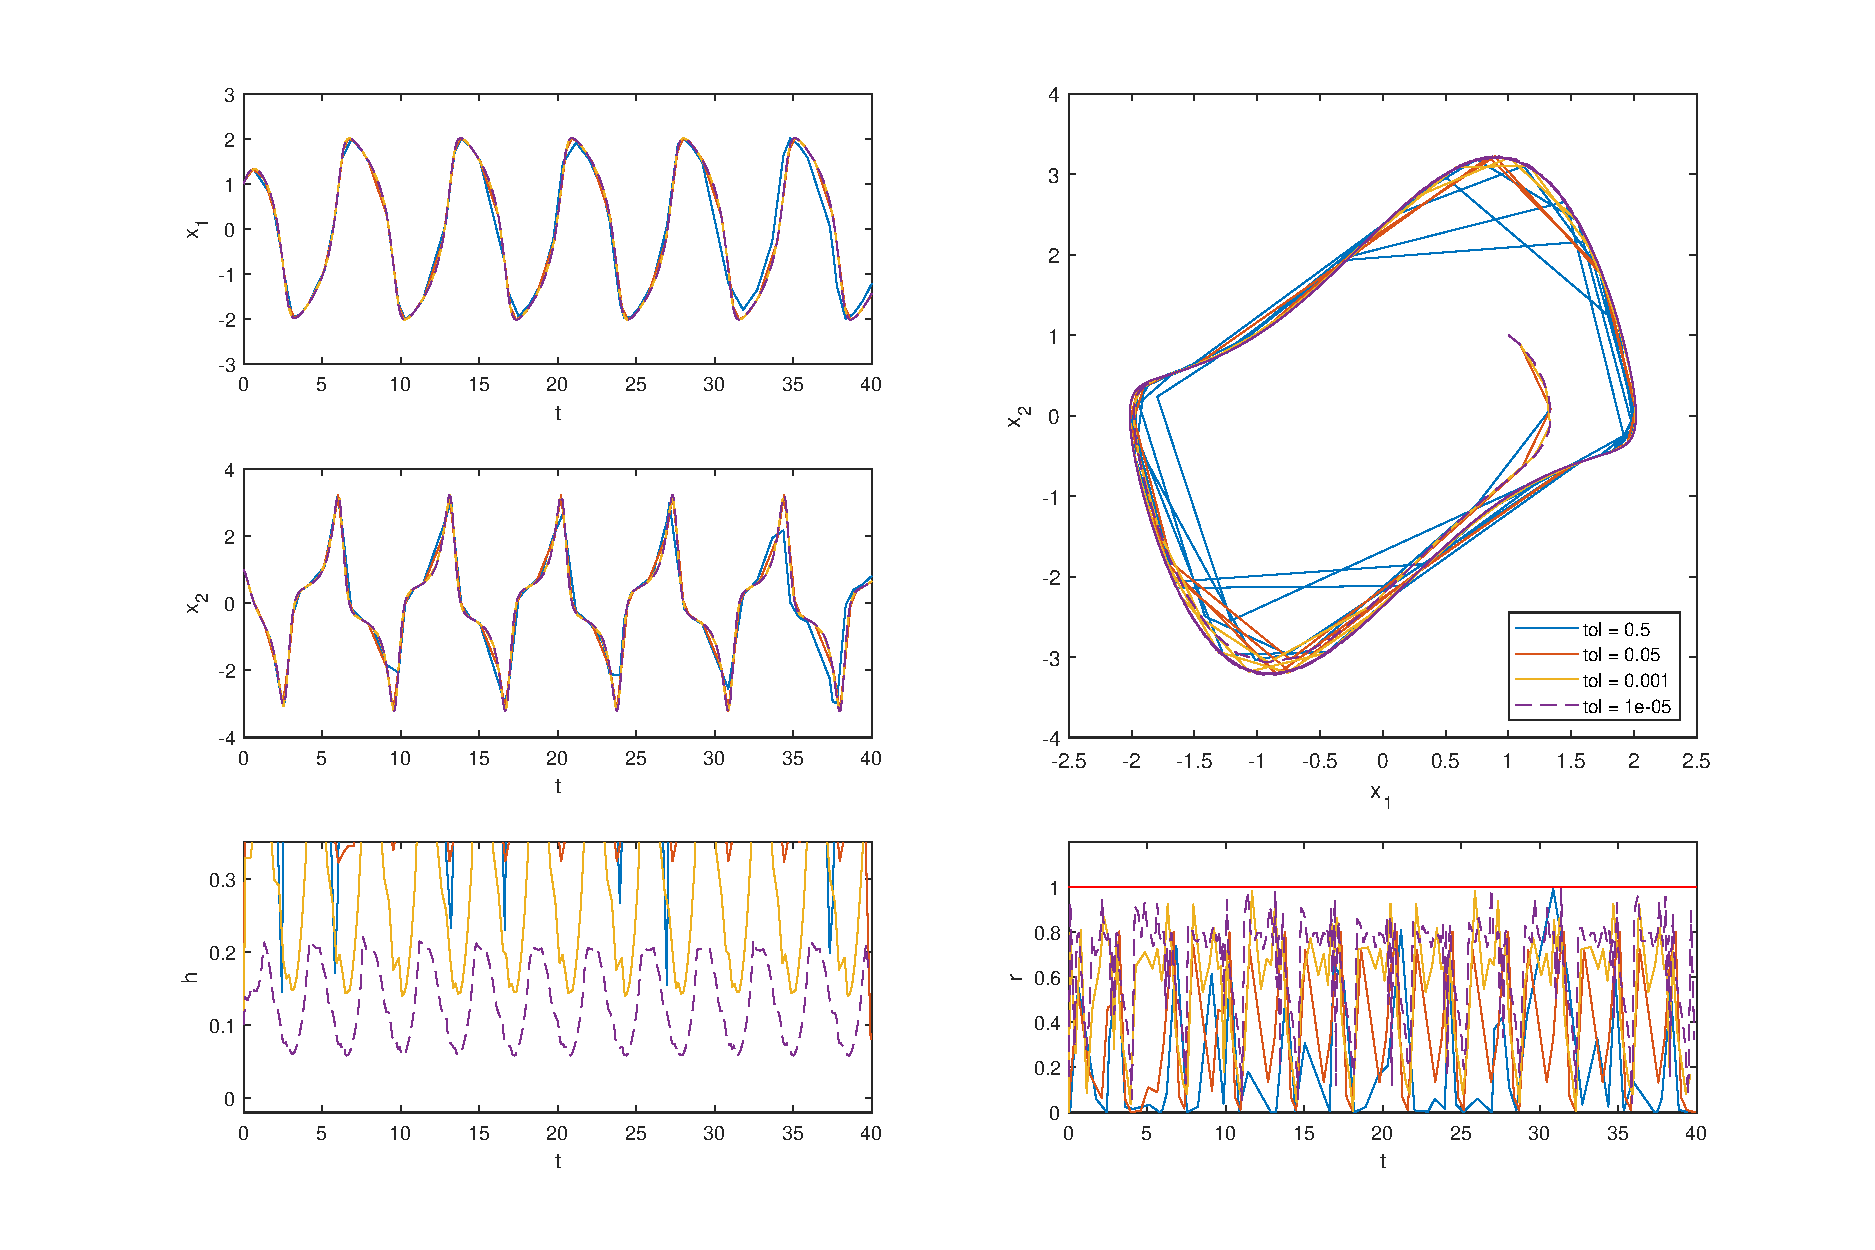
\includegraphics[width=1.25\textwidth]{images/6/6_4_adaptive_mu_1_5.pdf}}
    \caption{Solution for the Van der Pol problem ($\mathit{\mu = 1.5}$) using classical Runge-Kutta with adaptive step size}
    \label{6_4_RK4_mu_1_5}
\end{figure}

\begin{table}[H]
    \centering
    \begin{tabular}{@{}l|cccc@{}}
    \toprule
    Tolerances           & 0.5  & 0.05 & 0.001 & 1e-05 \\ \midrule
    Function evaluations & 1335 & 1690 & 2843  & 6440  \\
    Calculated steps     & 106  & 134  & 224   & 506   \\
    Accepted steps       & 63   & 82   & 155   & 368   \\
    Rejected steps       & 43   & 52   & 69    & 138   \\ \bottomrule
    \end{tabular}
    \caption{Parameters of the classical Runge-Kutta with adaptive step size for the Van der Pol problem ($\mathit{\mu = 1.5}$)}
    \label{6_4_adaptive_mu_1_5_table}
\end{table}

\begin{figure}[H]
    \centering
    \makebox[\textwidth][c]{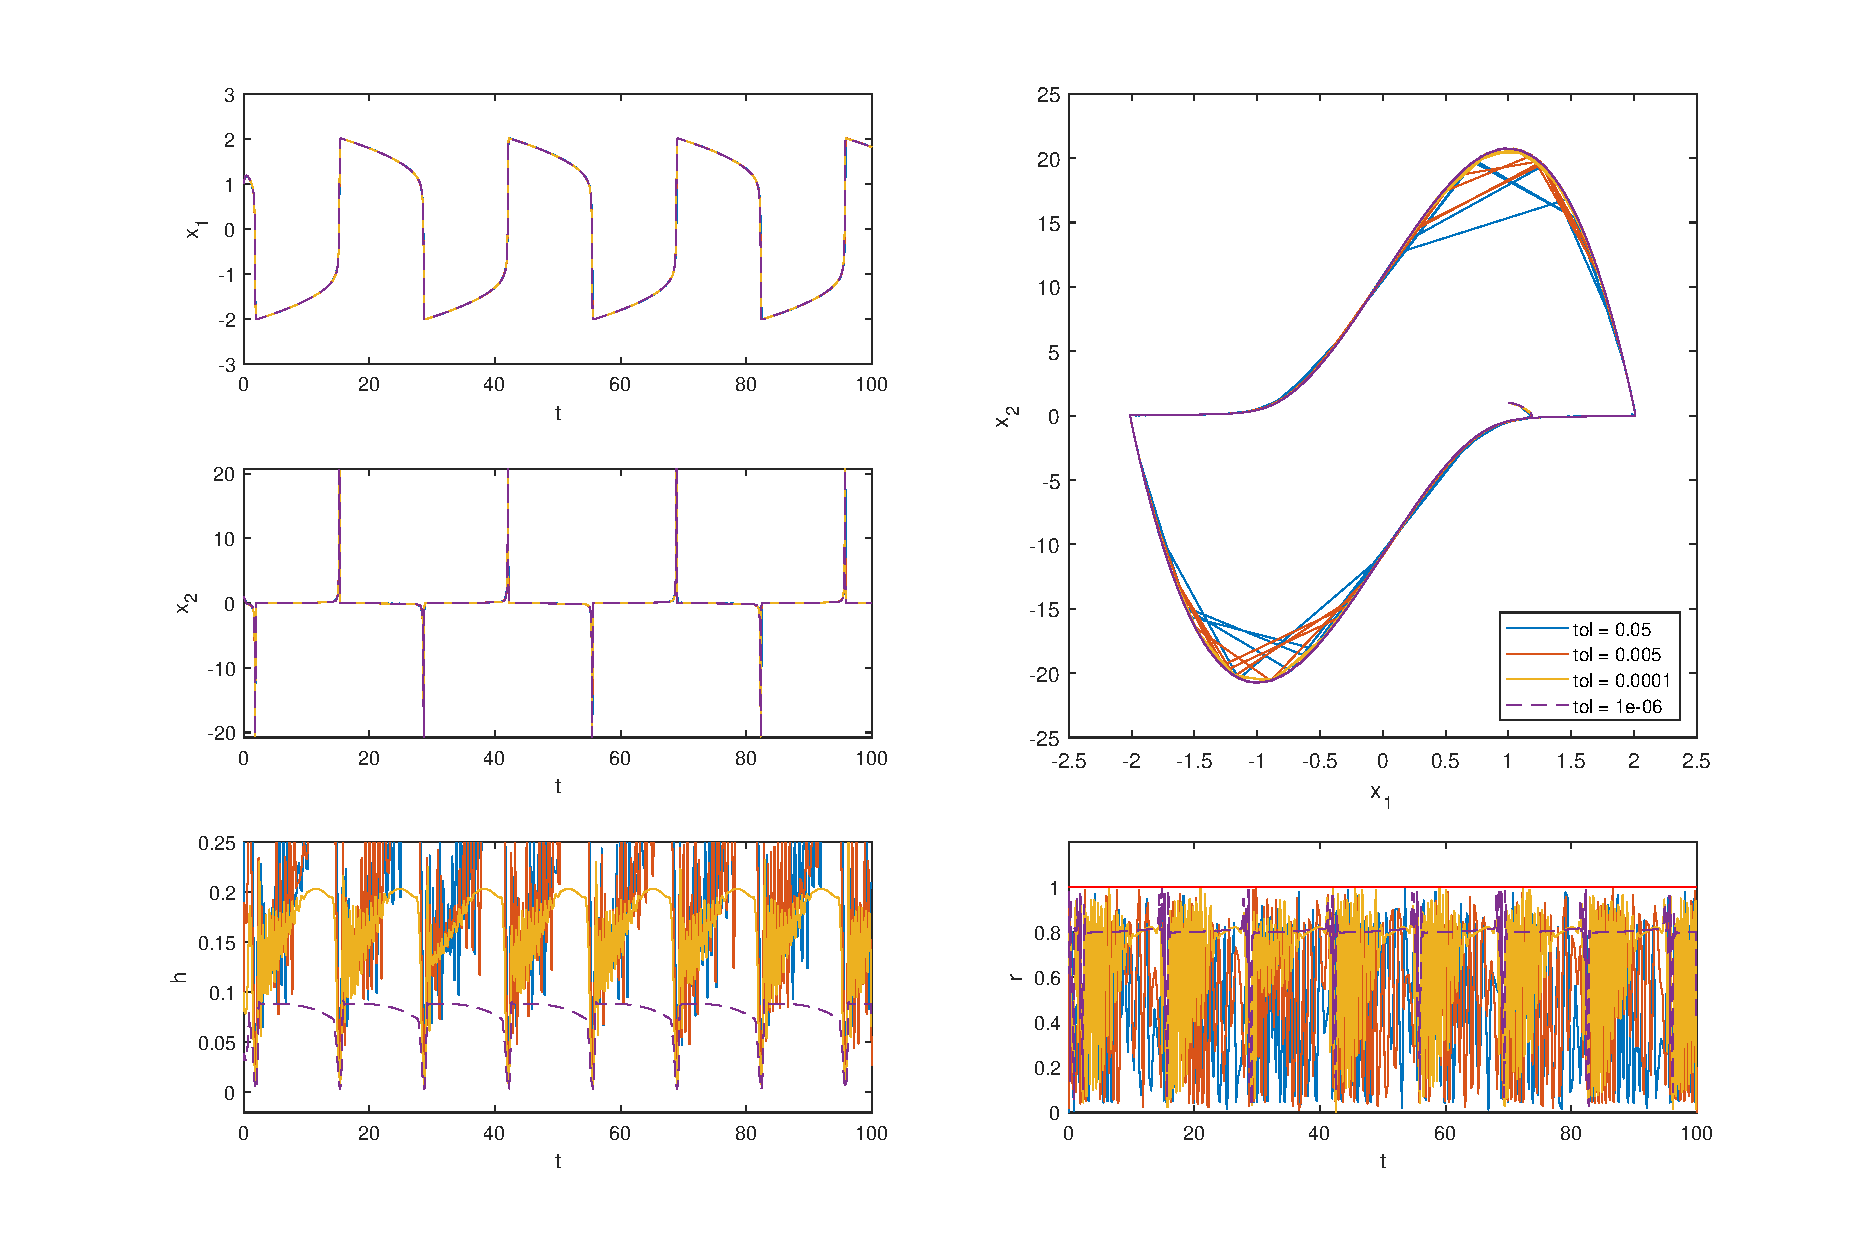
\includegraphics[width=1.25\textwidth]{images/6/6_4_adaptive_mu_15.pdf}}
    \caption{Solution for the Van der Pol problem ($\mathit{\mu = 15}$) using classical Runge-Kutta with adaptive step size}
    \label{6_4_RK4_mu_15}
\end{figure}

\begin{table}[H]
    \centering
    \begin{tabular}{@{}l|cccc@{}}
    \toprule
    Tolerances           & 0.05  & 0.005 & 0.0001 & 1e-06 \\ \midrule
    Function evaluations & 10951 & 11526 & 14814  & 26382 \\
    Calculated steps     & 867   & 910   & 1164   & 2050  \\
    Accepted steps       & 547   & 606   & 846    & 1782  \\
    Rejected steps       & 320   & 304   & 318    & 268   \\ \bottomrule
    \end{tabular}
    \caption{Parameters of the classical Runge-Kutta with adaptive step size for the Van der Pol problem ($\mathit{\mu = 15}$)}
    \label{6_4_adaptive_mu_15_table}
\end{table}

\pagebreak

%%%%%%%%%%%%%%%%%%%%%%%%%%%%%%%%%%%%%%%%%%%%%%%%%%%%%%%%%%%%%%%%%%%%%%%%%%%%%%%%%%%%%%%%%%%%%%%%%%%
\subsection{Test  your  algorithms  on  the  adiabatic  CSTR  problem  described  in  the papers uploaded to Learn (3D-version and 1D-version).}
Just as in the Van der Pol, the classical Runge-Kutta with adaptive step size manages to outperform the convergence achieved by the Explicit Euler. It also deals a lot better with the stiff area of the problem. However, even though it needs less steps to achieve a better solution with the same tolerance, the extra amount of function evaluations per step makes it only worthed when the tolerance is pretty small.

\begin{figure}[H]
    \centering
    \makebox[\textwidth][c]{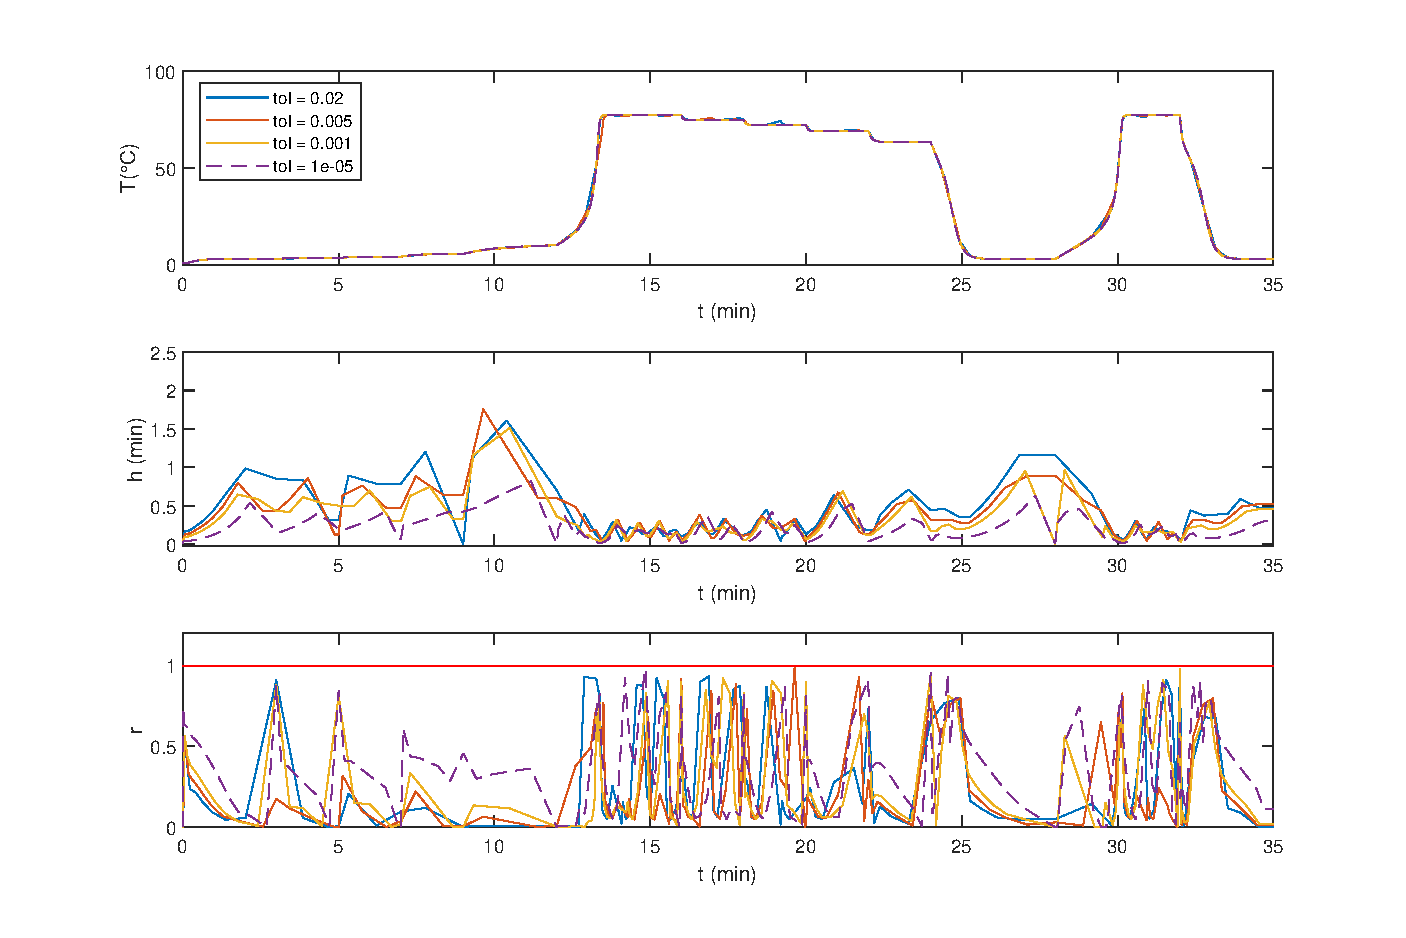
\includegraphics[width=1\textwidth]{images/6/6_5_3D_tols.pdf}}
    \caption{Solution for the CSTR 3D problem using classical Runge-Kutta with adaptive step size}
    \label{6_5_3D_tols}
\end{figure}

\begin{table}[H]
    \centering
    \begin{tabular}{@{}l|cccc@{}}
    \toprule
    Tolerances           & 0.02 & 0.005 & 0.001 & 1e-05 \\ \midrule
    Function evaluations & 2068 & 2168  & 2650  & 4274  \\
    Calculated steps     & 163  & 170   & 208   & 334   \\
    Accepted steps       & 112  & 128   & 154   & 266   \\
    Rejected steps       & 51   & 42    & 54    & 68    \\ \bottomrule
    \end{tabular}
    \caption{Parameters of the classical Runge-Kutta with adaptive step size for the CSTR 3D problem}
    \label{6_5_3D_tols_table}
\end{table}

\begin{figure}[H]
    \centering
    \makebox[\textwidth][c]{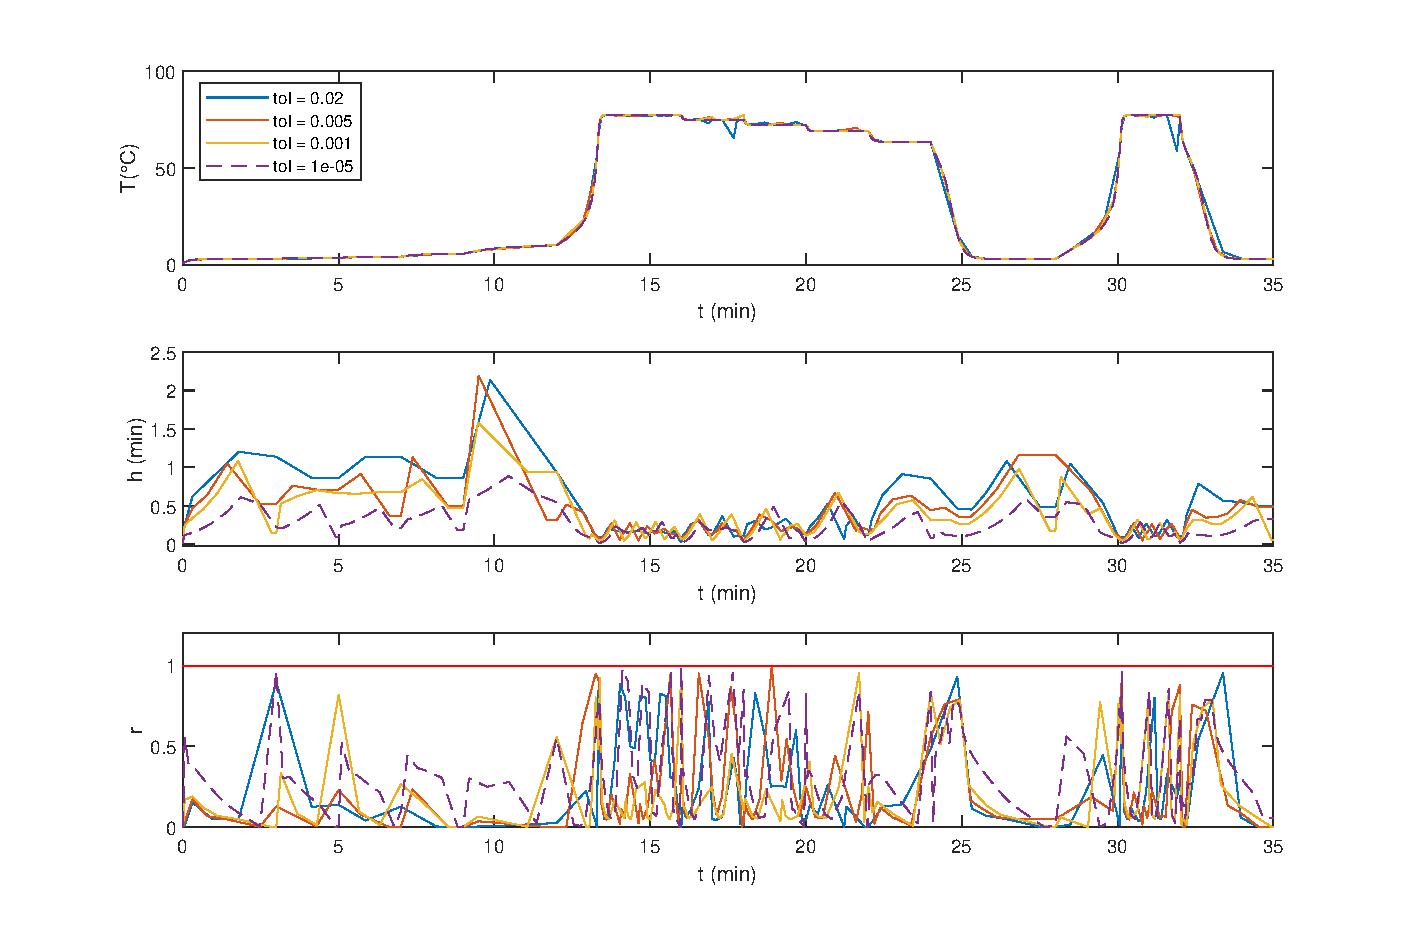
\includegraphics[width=1\textwidth]{images/6/6_5_1D_tols.pdf}}
    \caption{Solution for the CSTR 1D problem using classical Runge-Kutta with adaptive step size}
    \label{6_5_1D_tols}
\end{figure}

\begin{table}[H]
    \centering
    \begin{tabular}{@{}l|cccc@{}}
    \toprule
    Tolerances           & 0.02 & 0.005 & 0.001 & 1e-05 \\ \midrule
    Function evaluations & 1741 & 1909  & 2143  & 3425  \\
    Calculated steps     & 137  & 150   & 168   & 268   \\
    Accepted steps       & 97   & 109   & 127   & 209   \\
    Rejected steps       & 40   & 41    & 41    & 59    \\ \bottomrule
    \end{tabular}
    \caption{Parameters of the classical Runge-Kutta with adaptive step size for the CSTR 1D problem}
    \label{6_5_1D_tols_table}
\end{table}


%%%%%%%%%%%%%%%%%%%%%%%%%%%%%%%%%%%%%%%%%%%%%%%%%%%%%%%%%%%%%%%%%%%%%%%%%%%%%%%%%%%%%%%%%%%%%%%%%%%
\subsection{Compare the results from your algorithms with the results you get using some of Matlab's ODE solvers} \label{6_6}
For the Van der Pol problem, we tested the classical Runge-Kutta against \code{ode45} for the non-stiff case ($\mu = 1.5$), and against \code{ode15s} for the stiff case ($\mu = 15$). With this method, we are already approaching the ``big leagues" of ODE solvers. We can observe directly the effect that having a greater order of the error has on the solution: it's a lot more precise with big tolerances. Actually, the classical Runge-Kutta achieves similar accuracy to the \code{ode45}, when not better. However, this all comes with a cost, the number of function evaluations is also larger, but it's not as far from it as both Euler methods. As it's an explicit method, it doesn't stand a chance against the \code{ode15s} in the stiff case when looking at the number of function evaluations. However, the accuracy of the method is still surprisingly good, specially for low tolerances, where the \code{ode15s} misses the solution.

\begin{figure}[H]
    \centering
    \makebox[\textwidth][c]{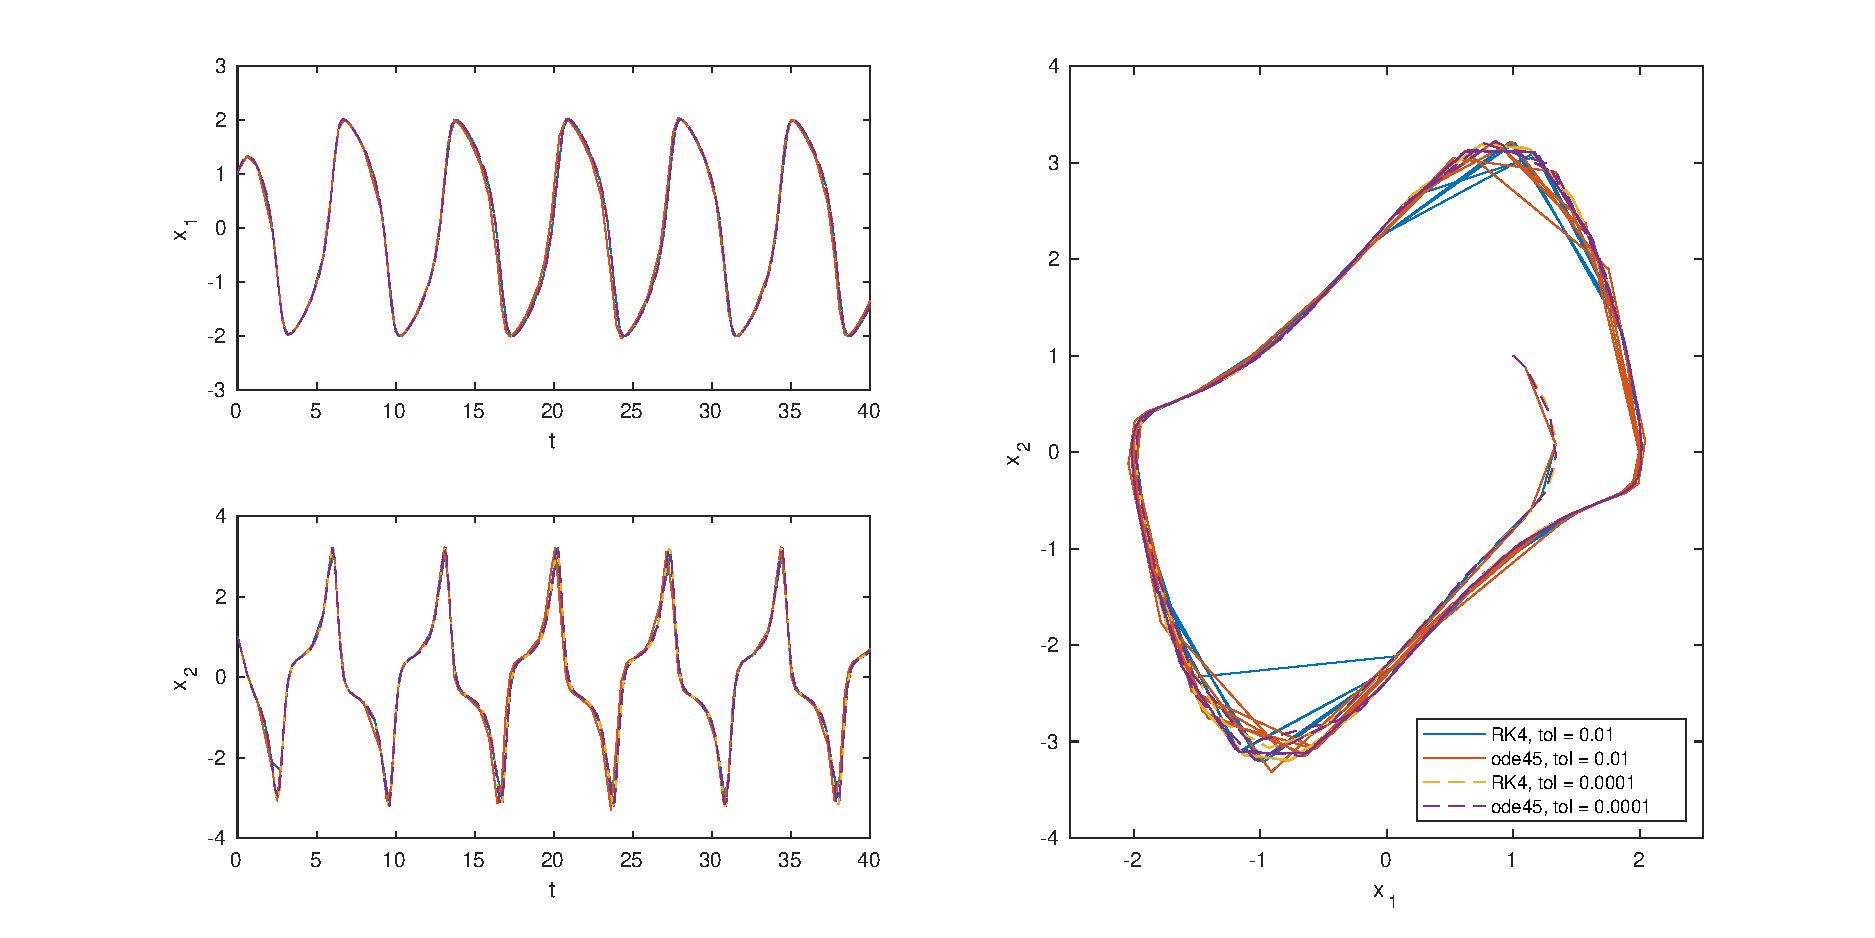
\includegraphics[width=1.25\textwidth]{images/6/6_6_mu_1_5.pdf}}
    \caption{Solution for the Van der Pol problem ($\mathit{\mu = 1.5}$) using Classical Runge-Kutta vs. \code{ode45}}
    \label{6_6_mu_1_5}
\end{figure}

\begin{table}[H]
    \centering
    \begin{tabular}{@{}l|cc|cc@{}}
    \toprule
    \textbf{Method}      & \multicolumn{2}{c|}{\textbf{RK4}} & \multicolumn{2}{c}{\textbf{ode45}} \\
    Tolerances           & 0.01           & 0.0001           & 0.01            & 0.0001           \\ \midrule
    Function evaluations & 2071           & 4341             & 787             & 1357             \\
    Calculated steps     & 164            & 342              & 131             & 226              \\
    Accepted steps       & 103            & 237              & 100             & 180              \\
    Rejected steps       & 61             & 105              & 31              & 46               \\ \bottomrule
    \end{tabular}
    \caption{Parameters of the Classical Runge-Kutta vs. \code{ode45} for the Van der Pol problem ($\mathit{\mu = 1.5}$)}
    \label{6_6_adaptive_mu_1_5_table}
\end{table}

\begin{figure}[H]
    \centering
    \makebox[\textwidth][c]{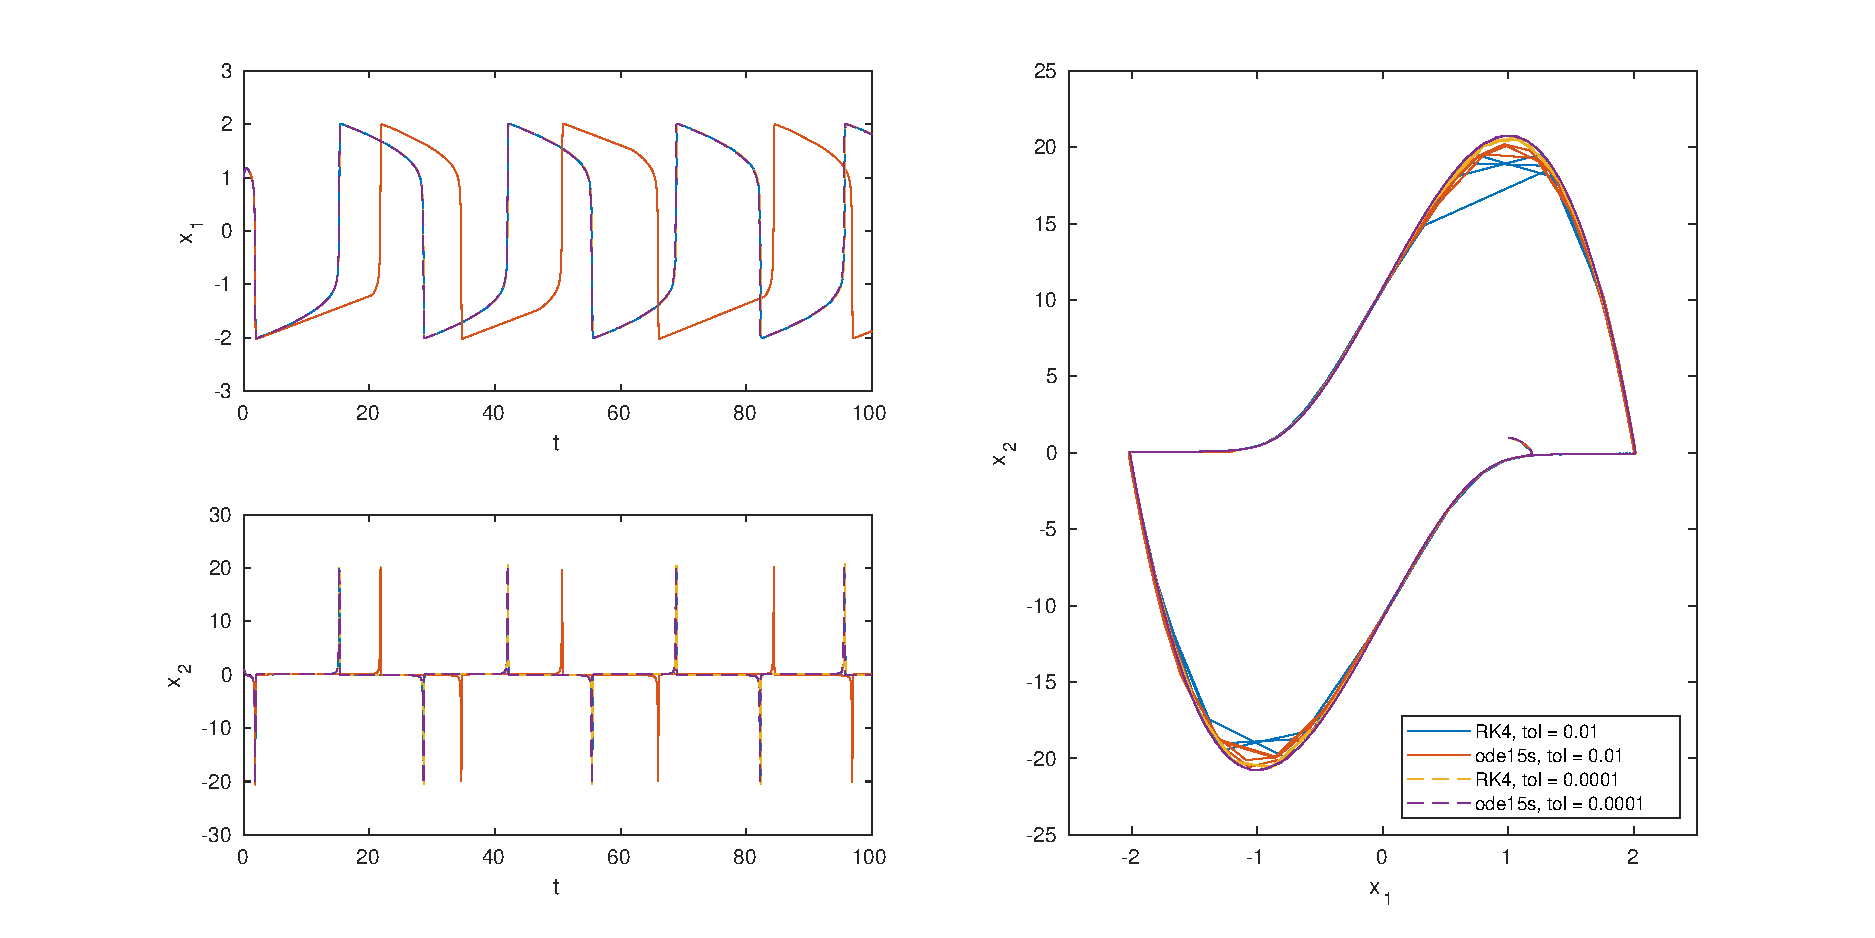
\includegraphics[width=1.25\textwidth]{images/6/6_6_mu_15.pdf}}
    \caption{Solution for the Van der Pol problem ($\mathit{\mu = 15}$) using Classical Runge-Kutta vs. \code{ode15s}}
    \label{6_6_mu_15}
\end{figure}

\begin{table}[H]
    \centering
    \begin{tabular}{@{}l|cc|cc@{}}
    \toprule
    \textbf{Method}      & \multicolumn{2}{c|}{\textbf{RK4}} & \multicolumn{2}{c}{\textbf{ode15s}} \\
    Tolerances           & 0.01            & 0.0001          & 0.01            & 0.0001            \\ \midrule
    Function evaluations & 11442           & 14814           & 1273            & 2780              \\
    Calculated steps     & 905             & 1164            & 558             & 1327              \\
    Accepted steps       & 582             & 846             & 411             & 1094              \\
    Rejected steps       & 323             & 318             & 147             & 233               \\ \bottomrule
    \end{tabular}
    \caption{Parameters of the Classical Runge-Kutta vs. \code{ode15s} for the Van der Pol problem ($\mathit{\mu = 15}$)}
    \label{6_6_adaptive_mu_15_table}
\end{table}

For the CSTR problem, we see how the three of them achieve good performance. The classical Runge-Kutta approaches the solution better that the \code{ode45}, but having more function evaluations. The \code{ode15s} continues to be the best one for this problem, specially in the 1D case.

\begin{figure}[H]
    \centering
    \begin{subfigure}{0.8\linewidth}
        \centering
        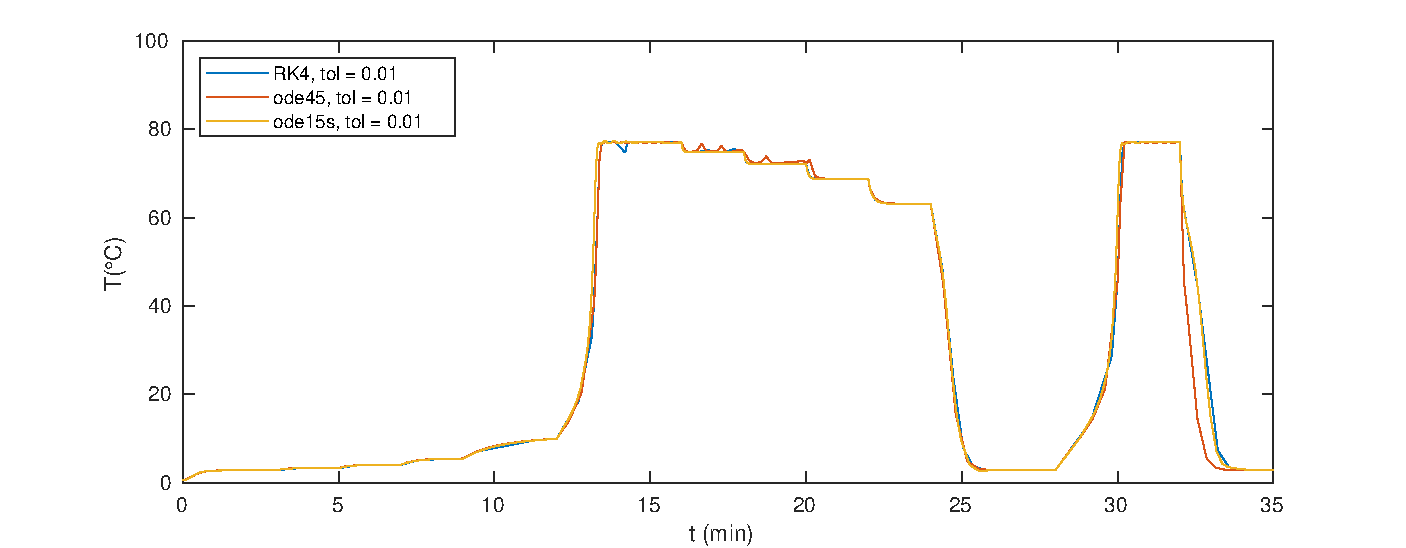
\includegraphics[width=1\linewidth]{images/6/6_6_3D.pdf} 
        \caption{CSTR 3D problem}
    \end{subfigure} \\
    \begin{subfigure}{0.8\linewidth}
        \centering
        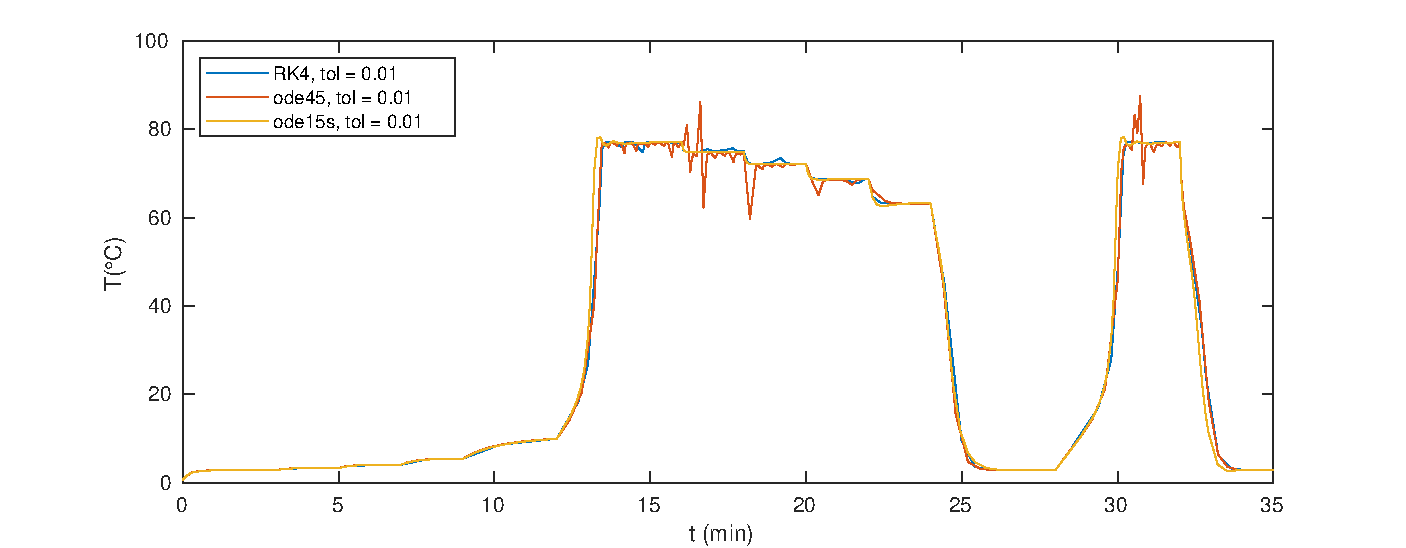
\includegraphics[width=1\linewidth]{images/6/6_6_1D.pdf}
        \caption{CSTR 1D problem}
    \end{subfigure}
    \caption{Solution for the CSTR problem using Classical Runge-Kutta vs. \code{ode45} and \code{ode15s}}
    \label{6_6_3D_1D}
\end{figure}

\begin{table}[H]
    \centering
    \begin{tabular}{@{}l|c|c|c@{}}
    \toprule
    \textbf{Method}      & \textbf{RK4} & \textbf{ode45} & \textbf{ode15s} \\
    Tolerances           & 0.01         & 0.01           & 0.01            \\ \midrule
    Function evaluations & 1978         & 1351           & 548             \\
    Calculated steps     & 155          & 1459           & 1612            \\
    Accepted steps       & 118          & 196            & 232             \\
    Rejected steps       & 37           & 27             & 36              \\ \bottomrule
    \end{tabular}
    \caption{Parameters of the Classical Runge-Kutta vs. \code{ode45} and \code{ode15s} for the CSTR-3D problem}
    \label{6_6_3D_table}
\end{table}

\begin{table}[H]
    \centering
    \begin{tabular}{@{}l|c|c|c@{}}
    \toprule
    \textbf{Method}      & \textbf{RK4} & \textbf{ode45} & \textbf{ode15s} \\
    Tolerances           & 0.01         & 0.01           & 0.01            \\ \midrule
    Function evaluations & 1906         & 1531           & 408             \\
    Calculated steps     & 150          & 1651           & 1316            \\
    Accepted steps       & 106          & 220            & 186             \\
    Rejected steps       & 44           & 33             & 30              \\ \bottomrule
    \end{tabular}
    \caption{Parameters of the Classical Runge-Kutta vs. \code{ode45} and \code{ode15s} for the CSTR-1D problem}
    \label{6_6_1D_table}
\end{table}


